\section{Analyzing filters for parallelizability}
Since the filters specify what the processing program should do to each row in a dataset, ``row by row'' or possibly chunks of rows is a suitable
granularity when implementing the parallelization of the program. Consequently, the filters of a file format are the prime candidates
for parallelization analysis. The analysis made is similar to the methodology used to identify the span in the work-span model described in
section \ref{work-span}. When applying the model to the problem of analyzing filters, a task is the processing of one row. In order to find
the tasks that need to be completed before other tasks, the filters that result in state that is accessed by subsequent rows or otherwise
affect the total processing of the dataset need to be identified.

Examining the filters, it is apparent that \textit{Dataset translation}, \textit{NullTranslationFilter}, \textit{Relation currency},
\textit{ThirdPartyAutomapper}, \textit{Set value}, \textit{RegExp extract}, and \textit{RegExp replace} only operate on the current dataset row, with no side effects.
This means that they produce no state changes that affect subsequent rows, which means that they do not affect the parallelizability of a dataset.

Additionally, \textit{Dataset information}, \textit{Tradefile information}, \textit{Temporary variable}, \textit{Logger}, and \textit{Skip row} perform
operations that either pull information from resources that are available to all rows, or produce an effect that does not affect any other rows.
The \textit{Conditional block} filter only produces effects according to its subfilters (a set of the filters already mentioned), and does not affect parallelization by itself.
\\\\
Hence, the filters that can affect the parallelization of a dataset are:
\begin{itemize}
  \item \textit{Mapping}, since the trade id mapping may need to keep track of state that can be accessed in subsequent rows in order to make all id:s unique.
  \item \textit{Header detection}, since all rows beneath the (first) header row depend on the column names for mappings and other values.
  \item \textit{Global variable}, since the variable may be written and accessed by any subsequent rows. Each rewrite of the variable needs to happen before the next rewrite,
    in the original, sequential order if the verification result is to be correct.
  \item \textit{State variable}, for the same reasons as Global variable.
  \item \textit{Stop processing}, if one thread sees a conditional fulfilled and stops processing, it is possible for another thread to keep processing rows that are intended
    to be ignored.
\end{itemize}

\section{Program overview} %TODO: Skriv om loggning
The general flow of the original, sequential, dataset processing program is the following:
\\\\
The unprocessed dataset has the rows stored in a Cassandra database, and some metadata and methods stored in a Django object backed by a MySQL database.
The file format corresponding to the dataset is looked up, and all of the filters it contains are added to a pipeline that will process the dataset.
An empty verification result is then created in both Cassandra and MySQL, containing the row data and result metadata with metrics, respectively.
The metrics include processing time, number of trades, timestamp, and similar data. The rows in the dataset are then processed one by one,
applying all filters to each row. As soon as a row has finished processing, it is written to the verification result in Cassandra.
During this process, the row mappings used in the \textit{Mapping} filter are fetched from the MySQL database, resulting in some
I/O waiting time. To mitigate this, the mappings are cached in memory for faster access. After the processing has finished, the result metadata
and metrics are saved in the MySQL database.

\section{Code inspection}
After an initial code and file format inspection, the following conclusions where made:
\begin{itemize}
  \item The \textit{Header detection} filter is effectively performed only once, as it is ignored for all rows after the one where the header was found.
  \item The filters \textit{Global variable} and \textit{State variable} make the processing of every row depend on the previous, as the writing of the variables may happen on each row.
  \item The process of making an ID unique could possibly be broken out to a post processing step.
  \item All file formats contain \textit{Header detection}, and many contain the make unique feature of the trade ID mapping.
  \item There are many file formats that do not have either \textit{Global variable}, \textit{State variable} or \textit{Stop processing} among their filters.
\end{itemize}

The conclusions above indicate that header detection may be done before creating the parallel processes, sending this data to each process when they are created.
If the process of producing unique ID:s is then done as a post processing step, the following task DAGs illustrate how the dependencies when processing different
file formats appear: In figure \ref{fig:embarrassing_dag}, the task DAG for a file format without a Global variable or State variable filter is illustrated.
In figure \ref{fig:embarrassing_dag}, the task DAG for a file format containing a Global variable is illustrated. Since the span is equal to the work
in the file formats containing Global variables or State variables, parallelization of datasets with these formats will result in no speedup according to the %Illustrate work-span?
work-span model (as $T_1 \leq T_\infty \Rightarrow S \leq 1$). File formats containing \textit{Stop processing} make it unfeasible to produce correct verification results
when parallelizing. Determination of whether the result is correct is non-viable if any rows are processed in different processes (as rows that should not be included in the result may be included anyway).

\begin{figure}[ht]
  \centering
  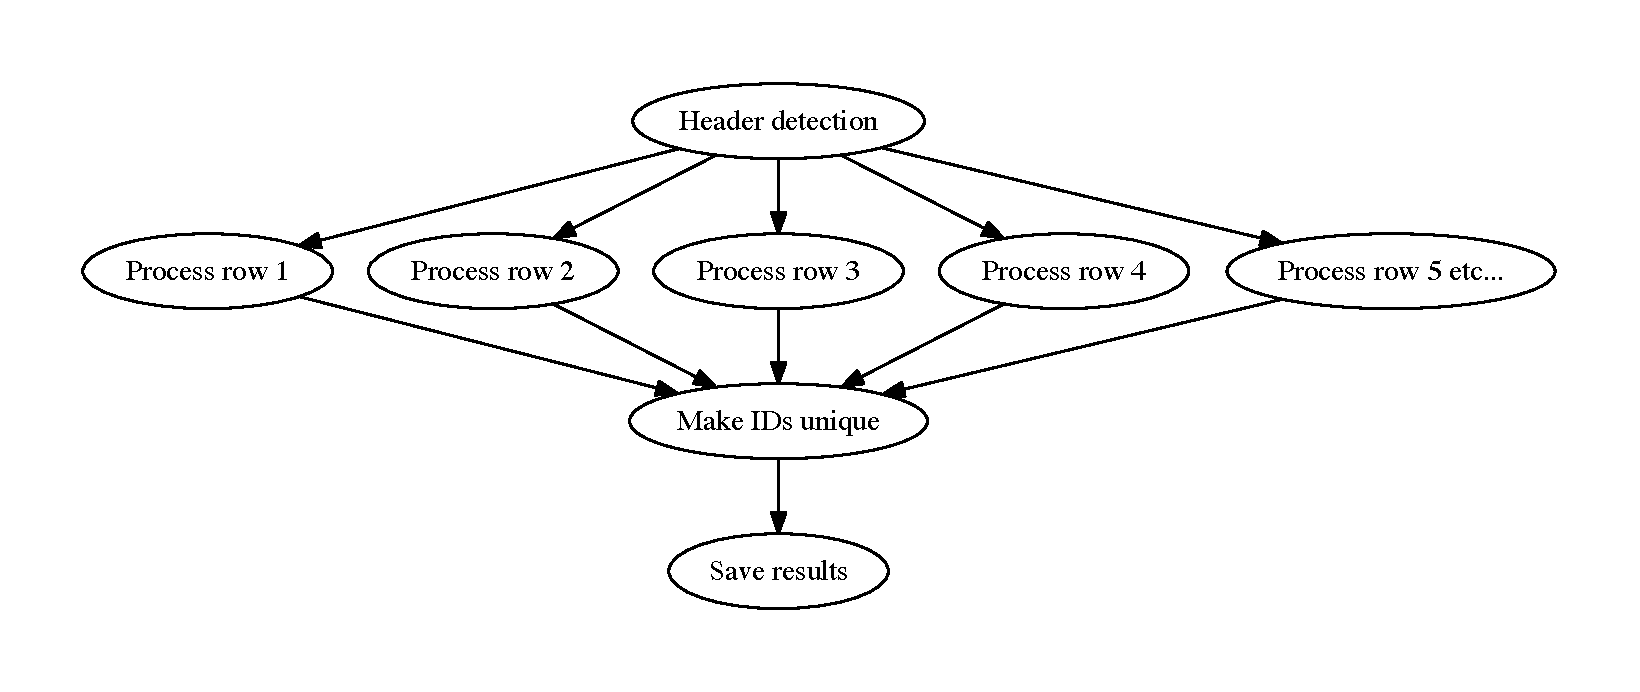
\includegraphics[width=120mm]{figures/embarrassing_file_format.pdf}
  \caption[Task DAG for a file format that does not contain global or state variables.]{An example of a task DAG for a file format that does not contain global variable or state variables. Header detections needs
  to be performed up front, and making trade IDs unique needs to be performed in a post processing step. The processing of each row does not depend on each other.}
  \label{fig:embarrassing_dag}
\end{figure}

\begin{figure}[ht]
  \centering
  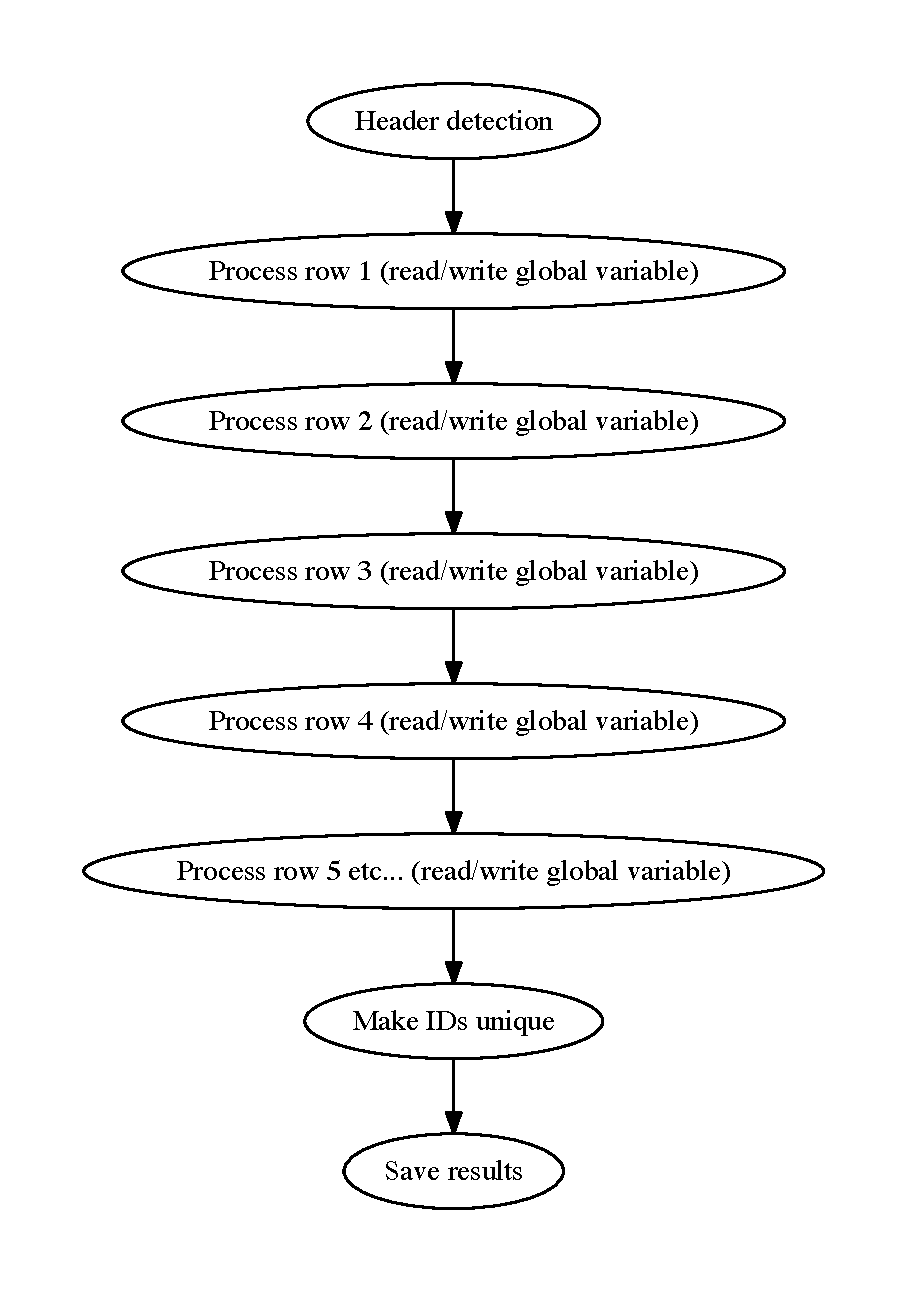
\includegraphics[width=120mm]{figures/global_variable_file_format.pdf}
  \caption[Task DAG for a file format that contains global or state variables.]{An example of a task DAG for a file format that contains global or state variables. Since each row may read and
  write the global (or state) variable, every task depends on the previous task.}
  \label{fig:global_dag}
\end{figure}

\section{Parallelization} %TODO: skriv om ordning i dataset
In accordance with section \ref{related_work}, the Python \code{multiprocessing} module was used to implement the parallelization of the program. Additionally, measures where taken to send as little
data as possible between processes and to avoid introducing excessive complexity to the codebase. The \code{multiprocessing.Queue} facility was chosen for communication between processes due to its
noted performance and built-in synchronization \cite{singh_2013_parallel_padpwprfmm}.

Before deciding to use the parallelized version of program, the list of filters in a file format is examined for \textit{Global variable}, \textit{State variable}, or \textit{Stop processing}. If any of these are found, the
program falls back to its sequential version. Otherwise, the program carries on in accordance with figure \ref{fig:embarrassing_dag}. First, before creating any additional processes, the Header detection filter
is applied row by row until it produces a result (commonly after a few rows). Next, a (tunable) number of processes, as well as two queues are created. A number of row spans, or chunks, are then created by splitting
the rows beneath the header row into equally sized partitions. The first queue is used to transfer the data needed to process a chunk of the dataset, including the header data, the row span, and the result metadata.
In order to avoid errors and sending large objects between processes, only the primary key used to retrieve the result metadata object from the MySQL database is sent to the processes.
After this, the processes can independently retrieve the data. The second queue is used for sending the partial metrics objects for each chunk, and for indicating if a process is done processing
its data or if it encountered an error. Since all other results are written to the Cassandra database, this is the only information that needs to be sent to the main process. The queues can be
denoted the 'chunk queue' and the 'message queue', respectively.

In each of the created processes, the rows in the chunk are retrieved from the Cassandra database and a new object containing metrics for the chunk is created. The chunk is then processed as in the sequential program,
applying all filters to each row. The metrics object is updated during the processing, as in the original program. If the chunk was processed correctly, the metrics object is put on the message queue. Otherwise,
if an exception occurs, an error message is put on the queue instead. When all data in a process has finished processing, a message indicating that the process has finished its work is put on the message queue.

The main process continuously polls the message queue, and merges the partial metrics objects as they are polled from the queue. If an error message is encountered, an exception is raised on the main thread, mimicking the
behavior of the original sequential program. It also increments a counter whenever a done message is received from a process. When the counter is equal to the number of subprocesses, the main process stops waiting
for messages, and progresses with the post processing step of making the trade ID:s unique. Finally, the main process saves the result object with the corresponding merged metrics to the MySQL database. At this point,
the program has produced a finished verification result.

\section{Sources of overhead}
During the implementation of the parallel version of the program, the following possible sources of parallelization overhead where identified:

\begin{itemize}
  \item The \code{multiprocessing} module, where creating processes and transferring data between processes is costly.
  \item Less effective caching. Since the mappings cache is local to each subprocess, caches are built up individually. This results in fewer cache hits than in the sequential program, and more total work
    looking up values in the MySQL database.
  \item The process of making trade ID:s unique is added as an extra step after the main data processing pipeline.
  \item Because of incompatibility with multiprocessing, the Python connections between both MySQL and Cassandra need to be restarted in the startup of each subprocess.
\end{itemize}
